\documentclass{book}
%\documentclass{article}

\usepackage{tikz}
\usetikzlibrary{external}
\usetikzlibrary{shapes}
\usetikzlibrary{fit}

\newcounter{a}
\newcounter{b}

\usepackage{braket}

\usepackage{subcaption} % Subfigure environment 
\usepackage{gensymb}

\usepackage{amsmath} % Mathematical symbols
\usepackage{amssymb} % Symbols

\usepackage{caption}% Captions onder figuur gecentreerd
%\usepackage[toc,page]{appendix}
\usepackage{subcaption} % Subfigure environment 
\usepackage{float}

\usepackage{etoolbox} %for if empty functionality

\usepackage{ifthen}

%break long urls at a - and not only at . or /
\usepackage{url}
\def\UrlBreaks{\do\/\do-}
\usepackage{breakurl}
\usepackage[hidelinks,breaklinks]{hyperref}

\usepackage{verbatim}
\usepackage{siunitx} % Elegant eenheden zetten
\usepackage[version=3]{mhchem} % ingeven van chemische fomules
\usepackage{cleveref} % Paragraaf tekens
\usepackage{longtable}
%\usepackage{lscape}
\usepackage[T1]{fontenc}
\usepackage{fontenc}
\usepackage{amsfonts}
\usepackage{mathtools}
\usepackage{grffile}%double dot in figure name
\usepackage{lipsum}
\usepackage{siunitx}
\usepackage{xcolor}
\usepackage{sectsty}
\usepackage{booktabs}
\usepackage{physics}
\usepackage{leftidx}
\usepackage[utf8]{inputenc}
\usepackage{gensymb} % /textdegree

\usepackage{epigraph}

\usepackage[toc,page]{appendix}

\usepackage{pdfpages}


% \tikzexternalize[prefix=tikz/]
% \tikzexternaldisable

%\setcounter{tocdepth}{4}
\setcounter{secnumdepth}{4}

\usepackage{graphicx}

\usepackage{todonotes}

%\usepackage[nottoc]{tocbibind}

\title{Thesis}

\date{2020}

\begin{document}

%\def\temp{#1}\ifx\temp\empty
%  <EMPTY>%
%\else
%  <NON EMPTY>%
%\fi




%use first argument is numbers of O's, second the labels, can be empty
%\mpo{3}{ {0,1,2,3,4} }

\newcommand{\combineTikz}[3]{
    \begin{tikzpicture}[baseline={0-0.5*height("$=$")}]
        \node (AA) at (0,0)  { #1   };
        \node (AB) at ( {#3} ,0)  {  #2  };
    \end{tikzpicture}
}


\newcommand{\mpo}[6]  { \begin{tikzpicture}[baseline={0-0.5*height("$=$")}]
        %\def \NNodes {#1}
        %\def \NodeName {#2}          
        %\def \NameUp   {#3} 
        %\def \NameDown  {#4}	

        \def \legLength {0.6}
        \def \radius {0.3}

        \pgfmathsetmacro{\step}{2*\radius+\legLength}
        \pgfmathsetmacro{\legpos}{\radius+\legLength}

        \pgfmathsetmacro{\Nmax}{#1-1}

        \foreach \N in {0,..., \Nmax }{
                \pgfmathsetmacro{\p}{\N*\step}

                % up and down labels
                \def\temp{#3}\ifx\temp\empty
                    \def \labelUp {}
                \else
                    \pgfmathsetmacro{\labelUp}{  {#3}[\N]  }
                \fi

                \def\tempp{#4}\ifx\tempp\empty
                    \def \labeldown {}
                \else
                    \pgfmathsetmacro{\labeldown}{  {#4}[\N]  }
                \fi


                \def\aab{#5}\ifx\aab\empty
                    \def \dotssite {0}
                \else
                    \pgfmathsetmacro{\dotssite}{  {#5}[\N]  }
                \fi

                \ifthenelse{\dotssite = 0}{

                    \def\aac{#6}\ifx\aac\empty
                        \def \nname {O}
                    \else
                        \pgfmathsetmacro{\nname}{  {#6}[\N]  }
                    \fi



                    \node[circle,draw, radius=\radius] (O\N) at (\p,0) {\nname};


                    \node[] (Ou\N) at (\p, \legpos ) { \labelUp };


                    \node[] (Od\N) at (\p,-\legpos) {\labeldown};


                    \draw (O\N) -- (Ou\N);
                    \draw (O\N) -- (Od\N);
                }{
                    \node[circle] (O\N) at (\p,0) { $\cdots$ };


                }


            }

        \ifthenelse{  #1  =1  }{}{
            \foreach \N in {1,...,\Nmax }{
                    \pgfmathsetmacro{\M}{\N-1}
                    \pgfmathsetmacro{\label}{ {#2}[\N]  }
                    %\pgfmathsetmacro{\label}{ 5}

                    \draw (O\M) --  node[above]  {\label} (O\N);
                }
        }

        \pgfmathsetmacro{\labelo}{ {#2}[0]}
        \pgfmathsetmacro{\labeli}{  {#2}[\Nmax+1]}

        \node (N0) at (-\legpos,0) {};
        \draw (N0) -- node[above] {\labelo} (O0);

        \pgfmathsetmacro{\endpos}{\step*\Nmax+\legpos}

        \node (Ne) at (\endpos,0) {};
        \draw (Ne) -- node[above] {\labeli} (O\Nmax);

        %\draw (O0) --  node[above] {1} (O1);


    \end{tikzpicture}}

\newcommand{\expH}[5]{ \begin{tikzpicture}[baseline={0-0.5*height("$=$")}]

        \def \NNodes {#1};


        \def\aaa{#2}\ifx\aaa\empty
            \def \text { $e^{-\beta \hat{H}_{\NNodes} }$ }
        \else
            \def \text {#2}
        \fi

        \pgfmathwidth{ "\text" }
        \def \textwidth { \pgfmathresult }


        %\pgfmathsetmacro{\text}{width(\text)}

        \def \legLength {0.6}
        \def \radius {0.3} %fix to fit text inside for size 1
        \def \boxHeight {0.4};

        \pgfmathsetmacro{\step}{2*\radius+\legLength}
        \pgfmathsetmacro{\legpos}{\radius+\legLength}
        \pgfmathsetmacro{\dotpos}{\boxHeight+\legLength/2}

        \pgfmathsetmacro{\Nmax}{\NNodes -1}



        \pgfmathsetmacro{\boxsize}{ max ( \textwidth/1cm , \step*\Nmax )   + \radius}

        %\pgfmathsetmacro{\boxsize}{ 5  )}
        %\pgfmathsetlength{\boxsize}{ max( \textwidth,  \boxsize1  )}



        %            \ifthenelse{#1=1}{
        %                \def \left {-0.6}
        %                \def \right {0.6}
        %            }{
        \def \left {-\radius}
        \def \right {\boxsize}
        %            }

        \draw (\left,- \boxHeight ) rectangle (\right, \boxHeight ) [add reference =H] ;


        \node  at (H center) { \text };

        \foreach \N in {0,..., \Nmax }{
                \pgfmathsetmacro{\p}{\N*\step}

                % up and down labels
                \def\temp{#3}\ifx\temp\empty
                    \def \labelUp {}
                \else
                    \pgfmathsetmacro{\labelUp}{  {#3}[\N]  }
                \fi

                \def\tempp{#4}\ifx\tempp\empty
                    \def \labeldown {}
                \else
                    \pgfmathsetmacro{\labeldown}{  {#4}[\N]  }
                \fi


                \node[] (O\N) at (\p,0) {};


                \ifthenelse{ \equal{\labelUp}{...}  }{
                    \node[] (Ou\N) at (\p, \dotpos ) {\labelUp};
                }{
                    \node[] (Ou\N) at (\p, \legpos ) {\labelUp};
                    \draw (Ou\N) --  (Ou\N  |- H north);
                }


                \ifthenelse{ \equal{\labeldown}{...}  }{
                    \node[] (Od\N) at (\p,-\dotpos ) {\labeldown};
                }{
                    \node[] (Od\N) at (\p,-\legpos) {\labeldown};
                    \draw (Od\N) --  (Od\N  |- H south);
                }
            }

        \def\tempt{#5}\ifx\tempt\empty

        \else
            \pgfmathsetmacro{\labelo}{ {#5}[0] }
            \pgfmathsetmacro{\labeli}{  {#5}[1] }

            \pgfmathsetmacro{\leftleg}{  \left - \legLength }
            \pgfmathsetmacro{\rightleg}{  \right + \legLength }

            \node (N0) at (\leftleg,0) {\labelo};
            \draw (N0) -- ( N0  -| H west);

            \node (Ne) at (\rightleg,0) {\labeli};
            \draw (Ne) --  ( Ne  -| H east);
        \fi


    \end{tikzpicture} }



% \begin{titlepage}
%   \begin{center}

%     \pagenumbering{gobble}
%     \includegraphics[width=4cm]{Figuren/UGent.png} \\[0.5cm]    %Logo UGENT	

%     \Large{\textsc{Master Engineering Physics}} \\[0.5cm]  %Vakgroep	

%     \normalsize{Year 2020-2021} \\[3cm]  %Academiejaar

%     \huge{\textsc{Master desertation}} \\[0.25cm]   %Titel

%     \Large{\textsc{Thesis Tensor networks}}\\[0.25cm]

%     \large \textnormal{October 2020} \\[2.5cm]   %Extra informatie

%     %\small      %Namen

%     David Devoogdt \\       [2.5cm]

%     Academic supervisor: prof.

%     \vfill

%   \end{center}
% \end{titlepage}

\frontmatter

%https://www.ugent.be/ea/nl/faculteit/studentenadministratie/masterproef/vorm1920.pdf

%\includepdf[page={1}]{ titelblad.pdf }

% \newpage
% \thispagestyle{empty}
% \mbox{}
% \newpage

\includepdf[page={1}]{ titelblad.pdf }

\newpage
\listoftodos
\newpage

%\twocolumn

\tikzset{add reference/.style={insert path={%
                    coordinate [pos=0,xshift=-0.5\pgflinewidth,yshift=-0.5\pgflinewidth] (#1 south west)
                    coordinate [pos=1,xshift=0.5\pgflinewidth,yshift=0.5\pgflinewidth]   (#1 north east)
                    coordinate [pos=.5] (#1 center)
                    (#1 south west |- #1 north east)     coordinate (#1 north west)
                    (#1 center     |- #1 north east)     coordinate (#1 north)
                    (#1 center     |- #1 south west)     coordinate (#1 south)
                    (#1 south west -| #1 north east)     coordinate (#1 south east)
                    (#1 center     -| #1 south west)     coordinate (#1 west)
                    (#1 center     -| #1 north east)     coordinate (#1 east)
                }}}

\addcontentsline{toc}{chapter}{Foreword}
\section*{Foreword}
\lipsum{20}

\section*{ Permission of use on loan }
The author(s) gives (give) permission to make this master dissertation available for consultation and to copy parts of this master dissertation for personal use. In all cases of other use, the copyright terms have to be respected, in particular with regard to the obligation to state explicitly the source when quoting results from this master dissertation.

\todo{add date}

\addcontentsline{toc}{chapter}{Abstract}

\section*{Abstract}

Het abstract is maximum één bladzijde en bevat minstens:
a) De informatie die werd vermeld op het titelblad (eigen vorm);
b) Een summiere beschrijving van het werk (vijftien à twintig regels);
c) Eventueel: drie tot vijf goed gekozen trefwoorden die het onderwerp best
omschrijven.

\addcontentsline{toc}{chapter}{Extended abstract}

\section*{Extended Abstract}

De extended abstract heeft een standaardlengte van minimaal twee bladzijden, met een maximum van zes bladzijden.

\tableofcontents

% \listoffigures

\mainmatter

\chapter{Introduction}

\epigraph{There is nothing new to be discovered in physics now. All that remains is more and more precise measurement.}{Lord Kelvin, 1900}

\todo{write this}

In 2015, there were about 5.6 million known physics papers in literature. At the current rate, this number doubles every 18.7 years \cite{Sinatra2015}. Despite this enormous body of literature, there are a lot of things which are not completely understood. Some examples include a self-consistent theory of quantum gravity, the need for dark energy and matter in cosmology, the arrow of time, the matter-antimatter asymmetry. There even is no interpretation of quantum mechanics where everyone agrees upon.

But certainly not all open problems have to do with 'new' physics. In many areas of physics, computing the implications of relatively simple laws becomes exceedingly difficult for many particles. Of historical importance is the three-body problem, describing the trajectory of 3 gravitational bodies such as the earth, moon and sun. The general case is not solved, despite developments over the last 300 years.

In reality, the real challenge is to model the macroscopic properties of quantum many-body system with around $10^{23}$ particles. Needless to say, this not an easy task at all. Finding good and computable approximations is of primary importance in the fields of quantum chemistry, condensed matter physics, and materials science.

In computational chemistry, the many-body problem is tackled with with methods which fall in one of the following categories: (post-) Hartree-Fock methods, density functional theory (DFT) and force-field methods. While they have many applications \todo{vind bron en voorbeelden}, these methods are not fully able to capture all the properties of the so called strongly correlated matter.

Examples of phase of strongly correlated matter which are not yet understood are include high-T superconductors, topological ordered phases, quantum spin liquids \cite{Orus2014}. There exist different methods to investigate these exciting materials. A very limited number of models is quantum integrable, meaning they can be solved in a non pertubative way. Also, some properties of models near criticality can be determined exactly with conformal field theory (CFT). But for some systems, we can only simulate the behaviour with numerical techniques.

%http://benasque.org/2020scs/talks_contr/106_tensornetworks_lecture1.pdf

To make progress in
strongly correlated
systems it is essential to
develop new accurate
numerical methods!
• DMFT / DCA
• Diagrammatic Monte Carlo
• Tensor network algorithms
• Fixed-node Monte Carlo
• Series expansion
• Density Matrix Embedding Theory
• Variational Monte Carlo
• Functional renormalization group
• Coupled-cluster methods

%

\chapter{Tensor networks}

The aim of this chapter is to give a basic introduction to tensor networks from a computational viewpoint. First the graphical notation for tensors, which is ubiquitous in the field, will be introduced and explained. A incomplete classification of the different kinds of tensor networks will be discussed. Some routine tensor network manipulations are explained. Also, a selection of different algorithms, which are from a computational point of view the reason behind the success of tensor networks, are presented very briefly.

\section{Tensor networks}

\subsection{introduction}

\subsubsection{graphical notation}
Tensor networks can be written in a graphical notation. The legs f a tensor denote the number of external indices. The upper  Connected legs are summed. Some examples are shown in \cref{tab:grafical_not}

\begin{table}[]
	\centering
	\caption{Caption}
	\begin{tabular}{l|l|l}
		conventional            & Einstein                & tensor notation           \\
		\hline
		$\Vec{x}$               & $x_{\alpha}$            &

		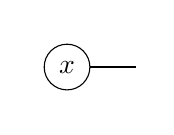
\begin{tikzpicture}[baseline=({N2.base}) ]
			\clip (-0.5,-0.5) rectangle (1,0.5);
			\node[circle, draw] (N2) at (0,0) {$x$};
			\node[] (N1) at (1,0) {};
			\draw  (N1) -- (N2) ;
		\end{tikzpicture}                                                     \\
		M                       & $M_{\alpha \beta}$      & 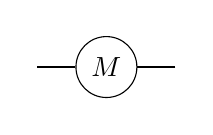
\begin{tikzpicture}[baseline={0cm-0.5*height("$=$")} ]
			\clip (-1,-0.5) rectangle (1,0.5);

			\node[circle, draw] (N2) at (0,0) {$M$};
			\node[] (N0) at (-1,0) {};
			\node[] (N1) at (1,0) {};

			\draw  (N1) -- (N2) ;
			\draw  (N0) -- (N2) ;

		\end{tikzpicture} \\

		$\Vec{x} \cdot \Vec{y}$ & $x_{\alpha} y_{\alpha}$ & 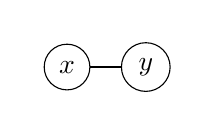
\begin{tikzpicture}[baseline=({N2.base}) ]
			\clip (-0.5,-0.5) rectangle (1.5,0.5);
			\node[circle, draw] (N2) at (0,0) {$x$};
			\node[circle, draw] (N1) at (1,0) {$y$};
			\draw  (N1) -- (N2) ;
		\end{tikzpicture} \\
	\end{tabular}

	\label{tab:grafical_not}
\end{table}

\subsection{Classification}

\paragraph{MPS}

A general quantum state with n sites can be described in a given basis $\ket{i}$ as
\begin{equation}
	\ket{\Psi} = \sum_{i_1 i_2 \cdots i_n } C^{i_1 i_2 \cdots i_n} \ket{i_1} \otimes \ket{i_2} \otimes \cdots \otimes \ket{i_n}
\end{equation}

This requires an exponential number $d^n$ of coefficients C where d is the dimensions of basis $\ket{i}$.

In order to make the problem tractable, the following form is proposed as wavefunction:

\begin{equation}
	C^{i_1 i_2 \cdots i_n} = {C^{1}}_{\alpha_1}^{ i_1} {C^{2}}_{\alpha_1 \alpha_2}^{i_2} \cdots  {C^{n}}_{\alpha_{n-1} }^{i_n}
\end{equation}
Where summation over shared indices is implied. It is always possible to find such an representation by means of matrix decomposition. The summation over $\alpha_i$ are called virtual bond and their dimension is denoted by $\chi$.

\begin{figure}
	\centering

	\begin{tikzpicture}[ ]

		\draw (-3,-0) rectangle (1,1)  [add reference=C]   ;
		\node  at (C center) {C};

		\node (N1)  at  (-2.5,-1) {};
		\node (N2)  at  (-1.5,-1) {};
		\node  at  (-.5,-0.5) {...};
		\node  (N3) at  (.5,-1) {};

		\draw    (N1) -- (N1 |-  C south);
		\draw    (N2) -- (N2 |-  C south);
		\draw    (N3) -- (N3 |-  C south);

	\end{tikzpicture}

	\caption{Caption}
	\label{fig:my_label}
\end{figure}

Explicit translational invariance is given by tensor $C^i_{\alpha \beta }$ that don't depend on the location. The chain is closed by setting $\alpha_n = \alpha_0$. We can now write this as a Trace over matrix products:

\begin{equation}
	\ket{\Psi} = \Tr( C^{i_1} C^{i_2} \cdots C^{i_n}  ) \ket{i_1} \otimes \ket{i_2} \otimes \cdots \otimes \ket{i_n}
\end{equation}

\missingfigure{make this in graphical notation}

\paragraph{MPO}

In a similar fashion, a Matrix Product Operator (MPO) is of the following form:

\begin{equation} \label{def_mpo}
	\begin{split}
		\hat{O} &= \sum Tr(A^{i_1 j_1} A^{i_2 j_2} \cdots A^{i_n j_n} M) \\
		& \times \ket{i_1}\bra{j_1} \otimes \ket{i_2}\bra{j_2} \otimes \cdots \otimes \ket{i_n}\bra{j_n}
	\end{split}
\end{equation}

\mpo{5}{{,,,,,}}{{"$i_1$","$i_2$",,"$i_n$","-"}}{{"$j_1$","$j_2$",,"$j_n$","-"}}{{0,0,1,0,0}}{{"A", "A",,"A","M" }}
\todo{connect trace and hide legs at M}

The matrix M contains the boundary conditions of the operator. Many Hamiltonians can be represented by an MPO. For ins

\paragraph{PEPS}

%https://arxiv.org/pdf/1306.2164.pdf
Exact contraction is hashtag P-Hard:

No exact canonical form

\paragraph{PEPO}

\paragraph{Others}

MERA,TTN,

\section{Tensor network manipulations}\label{sec:mpomath}
This section serves as an introduction of tensor network manipulations. The overview mainly focusses on MPS/MPO networks, but most of the oprations translate to the 2D case.

The MPS's are processed by transforming the tensor into a matrix, performing some matrix calculations and casting it back into its original form. In this way, the standard methods from linear algebra can be used. This section gives some examples how this is done in practice:

\subsection{Basics}

\subsubsection{Grouping legs}
One of the most basic manipulations is to group some legs of a tensor into one leg:
\begin{equation}
    \begin{split}
        T^{i_1 i_2 j_1 j_2} &=  \expH{2}{$T$}{{"$i_1$","$i_2$"}}{{"$j_1$","$j_1$"}}{} \\
        & \cong \expH{2}{$T$}{{"-","-"}}{{"-","-"}}{{"$(i_1 j_1 )$","$(i_2 j_2)$"}} \\
        &= T^{ (i_1 j_1 ) (i_2 j_2) } \\
    \end{split}
\end{equation}
The dimension of the new leg is the product of the dimension of the individual legs. Contracting 2 merged legs with 2 merged legs is exactly the same as contracting them separately. The both The 4 leg tensor and matrix contain exactly the same information.
Manipulating this in memory requires both permute and reshape commands. This requires some time, the internal representation of the matrix changes.

\subsubsection{decomposition} \label{decompMPO}

The grouping above can be applied to decompose a tensor into 2 tensor with matrix techniques. An example, which will be needed later on, is give here.

\def \figone {\expH{2}{$O^{u v,v w}$}{{"$i_1$","$i_2$"}}{{"$j_1$","$j_1$"}}{{"u","w"}}}

\begin{equation}
    \begin{split}
        \figone &= O^{i_1 i_2 j_1 j_2 }_{\alpha_u \gamma_w} \\
        &\cong O^{u w}_{ (\alpha_u i_1 j_1) (\gamma_w i_2 j_2) } \\
        &= O^{u v}_{(\alpha_u i_1 j_1) \alpha_v } O^{v w}_{ \alpha_v (\alpha_w i_2 j_2) } \\
        &\cong \mpo{2}{{"u","v","w"}}{{"$i_1$","$i_2$"}}{{"$j_1$","$j_1$"}}{}{}
    \end{split}
\end{equation}

The indices U,V and W represent blocks indices. Step 2 reshapes and groups the indices on to one index on the left and one on the right. The dimension of this index is the product of the separate dimensions. Step 3 decomposes the matrix into a product of 2 matrices. The last step transforms the indices back to separate legs.

For an exact representation, the bond dimension of virtual level v is:
\begin{equation}
    \dim{v} = \min( \dim{u}, \dim{v}) + 2 \dim{i}
\end{equation}

Many matrix decompositions exist. Some useful examples here are SVD decomposition, eigenvalue decomposition, QR, $\cdots$.

\subsubsection{virtual levels}
In the previous example, the levels were indicate with a block index or virtual level. The idea is to create seperate the contraction into blocks. This is completely analogous to matrix block multipliction. This wil be a more natural form to represent the algorithm. Of course, one can easily switch between block representation and the full one.

\subsubsection{inverse}
Suppose we want to find a MPO O for given tensors A and B such that the following holds:

\def \figone {\expH{2}{$A$}{{"$i_1$","$i_2$"}}{{"$j_1$","$j_2$"}}{{"u",}}}
\def \figthree {\expH{3}{$B$}{{"$i_1$","$i_2$","$i_3$"}}{{"$j_1$","$j_2$","$j_3$"}}{{"u","v"}}}

\def \figtwo {\mpo{1}{{,"v"}}{{"$i_3$",}}{{"$j_3$",}}{}{}}

\begin{equation}
    \combineTikz{ \figone }{\figtwo}{1.8} =  \figthree
\end{equation}

Again, the indices can be taken toghether in the following way: $\alpha = (u i_1 j_1  i_2 j_2)$ and $\beta = (i_3 j_3 v)$:
\begin{equation}
    A_{\alpha \gamma} O_{\gamma \beta} = B_{\alpha \beta}
\end{equation}
This a a standard matrix equation and can hence be solved with linear algebra packages. Note that it is not necessary to calculate $A^{-1}$ to obtain the solution. Linear solver are generally much faster. As this is one of the core problems to solve both in 1D and 2D, this will be discussed in detail in \cref{sec:framework_impl}.

\subsubsection{contraction order}

\todo{contraction order}

\subsubsection{Gauge freedom}

\todo{gauge}
\subsubsection{truncation}

\todo{svd truncation}

\subsection{MPS algoritms}

%https://arxiv.org/pdf/1306.2164.pdf

\subsubsection{cononical form}

schmidt decomp,

\subsubsection{DMRG}

\subsubsection{Expectation values}

Suppose that the there is an MPO representation of $ e^{ - \beta \hat{H} } $ A and that the mpo represenation for X Y is localised over n sites, then the expactation value is given by:

\begin{equation}
    \Braket{X} = \frac{
        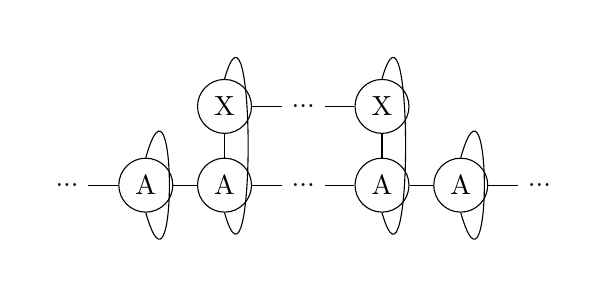
\begin{tikzpicture} [   ]
            \clip (-1.5,-1) rectangle (5.5,2);

            \node[] (N0) at (-1,0) {...};
            \node[circle, draw] (N1) at (0,0) {A};
            \node[circle, draw] (N2) at (1,0) {A};
            \node[circle, draw] (X2) at (1,1) {X};

            \node[] (N3) at (2 ,0) {...};
            \node[] (X3) at (2,1) {...};

            \node[circle, draw] (N4) at (3 ,0) {A};
            \node[circle, draw] (X4) at (3,1) {X};

            \node[circle, draw] (N5) at (4 ,0) {A};
            \node[] (N6) at (5 ,0) {...};

            \draw  (N0) -- (N1) ;

            \draw  (N1) -- (N2) ;
            \draw  (N2) -- (N3) ;
            \draw  (N3) -- (N4) ;
            \draw  (N4) -- (N5) ;
            \draw  (N5) -- (N6) ;

            \draw  (X2) -- (X3) ;
            \draw  (X3) -- (X4) ;

            \draw  (N2) -- (X2) ;
            \draw  (N4) -- (X4) ;

            \draw (X2.north)   .. controls +(0.4,1.4) and +(0.4,-1.4) .. (N2.south);
            \draw (X4.north)   .. controls +(0.4,1.4) and +(0.4,-1.4) .. (N4.south);

            \draw (N1.north)   .. controls +(0.4,1.4) and +(0.4,-1.4) .. (N1.south);
            \draw (N5.north)   ..  controls +(0.4,1.4) and +(0.4,-1.4)  .. (N5.south);
        \end{tikzpicture}
    }{
        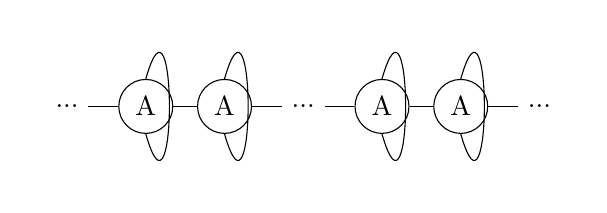
\begin{tikzpicture} [   ]

            \clip  (-1.5,-3) rectangle (5.5,-1);

            \node[] (O0) at (-1,-2) {...};
            \node[circle, draw] (O1) at (0,-2) {A};
            \node[circle, draw] (O2) at (1,-2) {A};

            \node[] (O3) at (2 ,-2) {...};
            \node[circle, draw] (O4) at (3 ,-2) {A};

            \node[circle, draw] (O5) at (4 ,-2) {A};
            \node[] (O6) at (5 ,-2) {...};

            \draw  (O0) -- (O1) ;

            \draw  (O1) -- (O2) ;
            \draw  (O2) -- (O3) ;
            \draw  (O3) -- (O4) ;
            \draw  (O4) -- (O5) ;
            \draw  (O5) -- (O6) ;

            \draw (O2.north)   .. controls +(0.4,1.4) and +(0.4,-1.4) .. (O2.south);
            \draw (O4.north)   .. controls +(0.4,1.4) and +(0.4,-1.4) .. (O4.south);

            \draw (O1.north)   .. controls +(0.4,1.4) and +(0.4,-1.4) .. (O1.south);
            \draw (O5.north)   ..  controls +(0.4,1.4) and +(0.4,-1.4)  .. (O5.south);
        \end{tikzpicture}
    }
    \label{sm:expecatation_X}
\end{equation}

In the thermodynamic limit there are an infinity number of A to the left and the right. This can be simulated by taking the left and right fixed points of the traced MPO A corresponding to the largest eigenvector $\lambda$.

\begin{equation}
    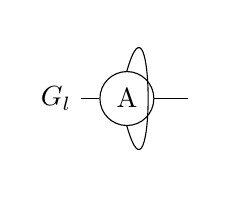
\begin{tikzpicture}[baseline={0cm-0.5*height("$=$")} , scale=0.9]
        \clip (-1.4,-1) rectangle (1,1);
        \node[] (N0) at (-1,0) {$G_l$};
        \node[] (N2) at (1,0) {};
        \node[circle, draw] (N1) at (0,0) {A};
        \draw  (N0) -- (N1) ;
        \draw  (N1) -- (N2) ;
        \draw (N1.north)   .. controls +(0.4,1.4) and +(0.4,-1.4) .. (N1.south);
    \end{tikzpicture}
    = \lambda
    \begin{tikzpicture}[baseline={0cm-0.5*height("$=$")}, scale=0.9 ]
        \clip (-.4,0.5) rectangle (1,-0.5);
        \node[] (N2) at (1,0) {};
        \node[] (N1) at (0,0) {$G_l$};
        \draw  (N1) -- (N2) ;
    \end{tikzpicture}
\end{equation}

\begin{equation}
    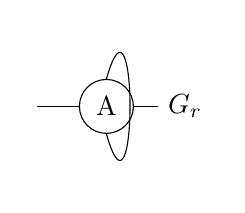
\begin{tikzpicture}[baseline={0cm-0.5*height("$=$")} ]
        \clip (-1,-1) rectangle (1.4,1);
        \node[] (N0) at (-1,0) {};
        \node[] (N2) at (1,0) {$G_r$};
        \node[circle, draw] (N1) at (0,0) {A};
        \draw  (N0) -- (N1) ;
        \draw  (N1) -- (N2) ;
        \draw (N1.north)   .. controls +(0.4,1.4) and +(0.4,-1.4) .. (N1.south);
    \end{tikzpicture}
    = \lambda
    \begin{tikzpicture}[baseline={0cm-0.5*height("$=$")} ]
        \clip (0,-0.5) rectangle (1.4,0.5);
        \node[] (N2) at (1,0) {$G_l$};
        \node[] (N1) at (0,0) {};
        \draw  (N1) -- (N2) ;
    \end{tikzpicture}
\end{equation}

Equation \cref{sm:expecatation_X} can now be easily caclulated:

\begin{equation}
    \Braket{X} = \frac{
        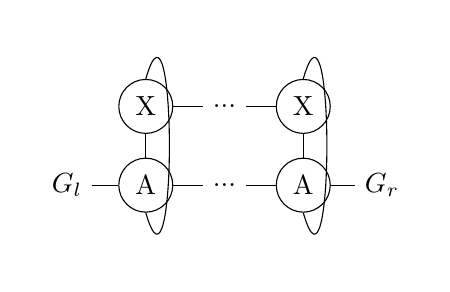
\begin{tikzpicture} [   ]
            \clip (-0.5,-1) rectangle (4.5,2);

            \node[] (N1) at (0,0) {$G_l$};
            \node[circle, draw] (N2) at (1,0) {A};
            \node[circle, draw] (X2) at (1,1) {X};

            \node[] (N3) at (2 ,0) {...};
            \node[] (X3) at (2,1) {...};

            \node[circle, draw] (N4) at (3 ,0) {A};
            \node[circle, draw] (X4) at (3,1) {X};

            \node[] (N5) at (4 ,0) {$G_r$};

            \draw  (N1) -- (N2) ;
            \draw  (N2) -- (N3) ;
            \draw  (N3) -- (N4) ;
            \draw  (N4) -- (N5) ;

            \draw  (X2) -- (X3) ;
            \draw  (X3) -- (X4) ;

            \draw  (N2) -- (X2) ;
            \draw  (N4) -- (X4) ;

            \draw (X2.north)   .. controls +(0.4,1.4) and +(0.4,-1.4) .. (N2.south);
            \draw (X4.north)   .. controls +(0.4,1.4) and +(0.4,-1.4) .. (N4.south);

        \end{tikzpicture}
    }{
        \lambda^n
        \begin{tikzpicture}[baseline={0cm-0.5*height("$=$")} ]
            \clip (-0.5,-0.5) rectangle (1.4,0.5);
            \node[] (N2) at (1,0) {$G_r$};
            \node[] (N1) at (0,0) {$G_r$};
            \draw  (N1) -- (N2) ;
        \end{tikzpicture}
    }
    \label{sm:expecatation_X_2}
\end{equation}



\section{Tensor network algorithms}

\section{MPS algorithms}

This section, and the following one, will introduce some different tensor network algorithms. The gaol is to provide an intuitive expanation how these algorithm work. For rigorous derivations and mathematical details, other sources can be read.

\subsection{Canonical form}

A translation invariant MPS has the following form:
\begin{equation}\label{mps:uni}
  \pepob{5}{2}{{
        "-","-", "-","-",
        "","","",""}}{{
        "-",
        "",
        "",
        "",
        "-"}}{{
        4,4,4,4,4,
        4,0,0,0,4}}
\end{equation}
It can be easily seen that inserting $X X^{-1}$ on each bond doesn't change the contracted tensor.
\begin{equation}
  A_l = \pepob{3}{2}{{
        "-","-",
        "",""}}{{
        "-",
        "",
        "-"}}{{
        4,4,4,
        4,2,4}}  =X \pepob{3}{2}{{
        "-","-",
        "",""}}{{
        "-",
        "",
        "-"}}{{
        4,4,4,
        4,0,4}} X^{-1}
\end{equation}

\begin{equation}
  A_r = \pepob{3}{2}{{
        "-","-",
        "",""}}{{
        "-",
        "",
        "-"}}{{
        4,4,4,
        4,3,4}}=Y \pepob{3}{2}{{
        "-","-",
        "",""}}{{
        "-",
        "",
        "-"}}{{
        4,4,4,
        4,0,4}} Y^{-1}
\end{equation}
and
\begin{equation}
  \pepob{3}{2}{{
        "-","-",
        "",""}}{{
        "-",
        "-",
        "-"}}{{
        4,4,4,
        4,6,4}}  = X Y^{-1} = C
\end{equation}
Then \cref{mps:uni}  can be written as follows:
\begin{equation}
  \pepob{6}{2}{{
        "-","-", "-","-","-",
        "","","","",""}}{{
        "-",
        "",
        "",
        "-",
        "",
        "-"}}{{
        4,4,4,4,4,4,
        4,2,2,6,3,4}}
\end{equation}
Introducing one more tensor:
\begin{equation}\label{algs:ACC}
  A_c = \pepob{3}{2}{{
        "-","-",
        "",""}}{{
        "-",
        "",
        "-"}}{{
        4,4,4,
        4,7,4}} = \pepob{4}{2}{{
        "-","-", "-",
        "","",""}}{{
        "-",
        "",
        "-",
        "-"}}{{
        4,4,4,4,
        4,2,6,4}} = \pepob{4}{2}{{
        "-","-", "-",
        "","",""}}{{
        "-",
        "-",
        "",
        "-"}}{{
        4,4,4,4,
        4,6,3,4}}
\end{equation}
At the moment the matrices $X$ and $Y$ are not yet defined. To bring an MPS A in its canonical form, the following choice is made

\begin{subequations} \label{algs:mpsid}
  \begin{alignat}{3}
                 & \vcenter{ \hbox{ \pepob{3}{2}{{
              "","",
              "",""}}{{
              "",
              "",
              "-"}}{{
              4,2,4,
    4,2,4}} } }= &                                 & \vcenter{ \hbox{  \pepob{3}{2}{{
              "","-",
              "","-"}}{{
              "",
              "-",
              "-"}}{{
              4,4,4,
    4,4,4}} } }  &                                 & = I                              \\
                 & \vcenter{ \hbox{ \pepob{3}{2}{{
              "","",
              "",""}}{{
              "-",
              "",
              ""}}{{
              4,3,4,
    4,3,4}} } }= &                                 & \vcenter{ \hbox{  \pepob{3}{2}{{
              "","-",
              "","-"}}{{
              "",
              "-",
              "-"}}{{
              4,4,4,
    4,4,4}} } }  &                                 & = I
  \end{alignat}
\end{subequations}

\todo{more on MPS}

\subsubsection{DMRG}

\section{2D tensor network contraction}

PEPS contraction concerns the following problem:
\begin{equation}\label{algs:biggrid}
  \rho_{i,j} =\vcenter{ \hbox{ \pepob{7}{7}{{
            "-","-", "-","-","-","-",
            "",  "", "","","","",
            "",  "", "","","","",
            "",  "", "","","","",
            "",  "", "","","","",
            "",  "", "","","","",
            "-", "-", "-","-","-","-",}}{{
            "-","-", "-","-","-","-",
            "","", "","","","",
            "","", "","","","",
            "","", "","","","",
            "","", "","","","",
            "","", "","","","",
            "-","-", "-","-","-","-",}}{{
            1,13,13,13,13,13,1,
            13,0,0,0,0,0,13,
            13,0,0,0,0,0,13,
            13,0,0,12,0,0,13,
            13,0,0,0,0,0,13,
            13,0,0,0,0,0,13,
            1,13,13,13,13,13,1,
          }} }}
\end{equation}
Contract an infinite lattice of identical tensors, with some irregularities on a small patch. For example, the one patch can be used to calculate an expectation value of a certain observable.

\subsection{Overview methods}

\subsubsection{Real-space renormalization-group methods}

\subsubsection{corner transfer matrix methods}

\subsubsection{Boundary methods}

\paragraph{  density-matrix renormalization group }

\paragraph{time-evolving block decimation }

\cite{Nietner2020}

\subsection{Vumps}

The porpuse of this section is to give some intuition on the variational uniform Matrix Product State  (VUMPS) algorithm, which will be used later on in this thesis.

The goal is to find a MPS layer for the MPO such that:
\begin{equation}\label{algs:mpslayermpo}
  \pepob{5}{3}{{
        "-","-", "-","-",
        "","","","",
        "","","","",}}{{
        "-", "-",
        "", "",
        "", "",
        "", "",
        "-", "-",}}{{
        4,4,4,4,4,
        13,0,0,0,13,
        13,2,7,3,13}}  \approx  \pepob{5}{2}{{
        "-","-", "-","-",
        "","","",""}}{{
        "-",
        "",
        "",
        "",
        "-"}}{{
        4,4,4,4,4,
        13,2,7,3,13}}
\end{equation}
This is very similar to \cref{algs:exp}. The expression holds approximately, because the MPS on the left hand side has a larger bond dimension than on the right hand side.

\subsubsection{The equations}
Suppose there are tensor which fullfil the conditions stated below:
\begin{subequations} \label{algs:vumpsenv}
  \begin{alignat}{2}
                             & \vcenter{ \hbox{  \pepob{5}{3}{{
              "","-", "-","",
              "","Gl","","",
              "","","",""}}{{
              "-","-",
              "-","-",
              "","",
              "-","-",
              "",""}}{{
              1,4,4,4,1,
              1,4,0,4,1,
    1,5,2,4,1}} }} = \lambda &                                   & \vcenter{ \hbox{    \pepob{5}{3}{{
              "-","-", "-","-",
              "-","","Gl","-",
              "-","","","-"}}{{
              "-","-",
              "-","-",
              "","",
              "-","-",
              "-","-"}}{{
              1,4,4,4,1,
              1,4,2,4,1,
    1,1,5,4,1}}}}                                                                                     \\
                             & \vcenter{ \hbox{   \pepob{5}{3}{{
              "-","-", "-","-",
              "","","Gr","-",
              "","","",""}}{{
              "-","-",
              "-","-",
              "","",
              "-","-",
              "-","-"}}{{
              1,4,4,4,1,
              1,4,0,4,1,
    1,4,8,1,1}} }}=  \lambda &                                   & \vcenter{ \hbox{ \pepob{5}{3}{{
              "-","-", "-","-",
              "-","-","Gr","",
              "-","-","",""}}{{
              "-","-",
              "-","-",
              "-","-",
              "","",
              "-","-"}}{{
              1,1,4,4,4,
              1,1,4,3,4,
              1,1,10,1,1}} }}
  \end{alignat}
\end{subequations}

These eigentensor equations are solved in pratice in a slightly different manner:
\begin{equation}\label{vumps_transfer_eigs}
  \vcenter{ \hbox{   \pepob{5}{3}{{
            "-","", "","-",
            "","","Gr","-",
            "","","",""}}{{
            "-","-",
            "-","-",
            "","",
            "","",
            "-","-"}}{{
            1,4,3,4,1,
            1,4,0,4,1,
            1,4,8,1,1}} }}=  \lambda  \vcenter{ \hbox{ \pepob{5}{3}{{
            "-","", "","",
            "-","-","Gr","",
            "-","-","",""}}{{
            "-","-",
            "-","-",
            "-","-",
            "","",
            "",""}}{{
            1,1,4,4,1,
            1,1,4,4,1,
            1,1,10,1,1}} }}
\end{equation}
Wher the $ Ar  $ tensor was connected from below on both sides and \cref{algs:mpsid} was used on the right hand side. The blocks in \cref{algs:vumpsenv} form a zipper from the left and right respectively. Each application brings down one of the MPS tensors in the following way.
\begin{equation}
  \begin{split}
    &       \vcenter{ \hbox{ \pepob{7}{3}{{
              "-","-", "-","-","-","-",
              "","Gl","","","","",
              "","","","","","",}}{{
              "-", "-",
              "", "",
              "", "",
              "", "",
              "", "",
              "", "",
              "-", "-",}}{{
              1,4,4,4,4,4,4,
              13,2,0,0,0,0,13,
              1,5,2,2,2,2,13}}}} \\
    =&       \vcenter{ \hbox{ \pepob{7}{3}{{
              "-","-", "-","-","-","-",
              "","","Gl","","","",
              "","","","","","",}}{{
              "-", "-",
              "", "",
              "", "",
              "", "",
              "", "",
              "", "",
              "-", "-",}}{{
              1,4,4,4,4,4,4,
              13,2,2,0,0,0,13,
              1,1,5,2,2,2,13}}}} \\
    =&       \vcenter{ \hbox{ \pepob{7}{3}{{
              "-","-", "-","-","-","-",
              "","","","Gl","","",
              "","","","","","",}}{{
              "-", "-",
              "", "",
              "", "",
              "", "",
              "", "",
              "", "",
              "-", "-",}}{{
              1,4,4,4,4,4,4,
              13,2,2,2,0,0,13,
              1,1,1,5,2,2,13}}}} \\
  \end{split}
\end{equation}
The left and right zipper can now move towards each other, until they meet at the center. In order to become the same MPS as before the application to the MPO (\cref{algs:mpslayermpo}), one more condition is needed:
\begin{equation} \label{algs:AC}
  \vcenter{ \hbox{   \pepob{5}{3}{{
            "-","-", "-","-",
            "","Gl","Gr","-",
            "","","",""}}{{
            "-","-",
            "-","-",
            "","",
            "-","-",
            "-","-"}}{{
            1,4,4,4,1,
            1,4,0,4,1,
            1,5,9,1,1}} }}=  \lambda  \pepob{3}{2}{{
        "-","-",
        "",""}}{{
        "-",
        "",
        "-"}}{{
        4,4,4,
        4,7,4}}
\end{equation}
This completely determines the problem, but one more equation is used to solve the problem. Combining on of the equations \cref{algs:vumpsenv}, the definitipn of $A_c$ \cref{algs:AC} and one of \cref{algs:mpsid} gives $C$:
\begin{equation}\label{algs:vumpsenvc}
  \vcenter{ \hbox{   \pepob{5}{3}{{
            "-","-", "-","-",
            "","Gl","Gr","-",
            "","","",""}}{{
            "-","-",
            "-","-",
            "-","-",
            "-","-",
            "-","-"}}{{
            1,4,4,4,1,
            1,4,4,4,1,
            1,5,11,1,1}} }}  =  \lambda  \pepob{3}{2}{{
        "-","-",
        "",""}}{{
        "-",
        "-",
        "-"}}{{
        4,4,4,
        4,6,4}}
\end{equation}
\todo{fix gap}

Then  \cref{algs:mpslayermpo} is solved:

\begin{equation}
  \begin{split}
    & \vcenter{ \hbox{ \pepob{7}{3}{{
              "-","-", "-","-","-","-",
              "","","","","","",
              "","","","","","",}}{{
              "-", "-",
              "", "",
              "", "",
              "", "",
              "", "",
              "", "",
              "-", "-",}}{{
              4,4,4,4,4,4,4,
              13,0,0,0,0,0,13,
              13,2,2,7,3,3,13}} }}\\
    &=       \vcenter{ \hbox{ \pepob{7}{3}{{
              "-","-", "-","-","-","-",
              "","Gl","","","Gr","",
              "","","","","","",}}{{
              "-", "-",
              "", "",
              "", "",
              "", "",
              "", "",
              "", "",
              "-", "-",}}{{
              1,4,4,4,4,4,4,
              13,2,0,0,0,3,13,
              1,5,2,7,8,1,4}}}} \\
    &=  \vcenter{ \hbox{ \pepob{7}{3}{{
              "-","-", "-","-","-","-",
              "","","Gl","Gr","","",
              "","","","","","",}}{{
              "-", "-",
              "", "",
              "", "",
              "", "",
              "", "",
              "", "",
              "-", "-",}}{{
              1,4,4,4,4,4,4,
              13,2,2,0,3,3,13,
              1,1,5,9,1,1,1}} }}\\
    &= \vcenter{ \hbox{ \pepob{7}{3}{{
              "-","-", "-","-","-","-",
              "","","","","","",
              "","","","","","",}}{{
              "-", "-",
              "", "",
              "", "",
              "", "",
              "", "",
              "", "",
              "-", "-",}}{{
              1,4,4,4,4,4,4,
              13,2,2,7,3,3,13,
              1,1,1,1,1,1,1}} }}
  \end{split}
\end{equation}

\todo{check lambdas in literature}

Contracting a 2D tensor network is thus reduced to solving the  \cref{algs:ACC}, \cref{algs:vumpsenv}, \cref{algs:AC} and \cref{algs:vumpsenvc} simultaneously. Inspection of the equations show that the following cycle needs to be solved:

\begin{itemize}
  \item  $A_c,C  \rightarrow A_l,A_r  $  \cref{algs:ACC}
  \item  $A_l,A_r  \rightarrow G_l,G_r  $ \cref{algs:vumpsenv}
  \item  $ G_l,G_r   \rightarrow Ac,C $ \cref{algs:AC} and  \cref{algs:vumpsenvc}
\end{itemize}

The calculated environment can now be used to solve the original problem. Due to symmetry, the same MPS can be applied from below. \cref{algs:vumpsenvc} now becomes:
\begin{equation}
  \vcenter{ \hbox{   \pepob{5}{3}{{
            "","", "","",
            "","Gl","Gr","",
            "","","",""}}{{
            "-","-",
            "","",
            "","",
            "","",
            "-","-"}}{{
            13,2,7,3,13,
            13,2,4,3,13,
            1,5,9,1,1}} }}
\end{equation}

\subsubsection{The derivation}\label{vumps_Deriv}
While the above derivation is reasonable, it is not very rigorous. The algorithm finds its origins  in tangent space methods, such as explained in \cite{Vanderstraeten2019}.

Not every state in the many body Hillbert space can be represented by an MPS. For a

By carefully constructing the tangent space and making use of the available gauge freedom, a compact expression can be found for the tangent space projector $\mathcal{P}_A$. This projects a state from the many body Hillbert space to the tangent space of an MPS A. For an optimal MPS approximation A, the error made in the approximation should be orthogonal to the tangent space. For \cref{algs:mpslayermpo} this means that the application of the projection of the error on the tangent space should be zero, i.e. the MPS is at a variational minimum.  \cite{Nietner2020}

Applying the projector $\mathcal{P}_A$ to \cref{algs:mpslayermpo} exactly gives rise to the equations stated earlier.



\chapter{Strongly correlated matter}

\section{Phases and Criticality} \label{sec:PhasesAndCrit}
\todo(scale invariancem, critical points, universality,critical exponents)

\section{Models}
\subsection{Ising model}

\subsubsection{Classical Ising}

The classical ising model is given by the following hamiltonian:
\begin{equation}
    H = -J \left (  \sum_{<i j>} \sigma_i \sigma_j + g\sum_i \sigma_i \right )
\end{equation}
where $<i j>$ runs over all neighbouring lattice sites. Classical refers to the fact that all the operators in the hamiltonian commute with each other. The values of $\sigma$ depends on the spin dimension. For spin $1/2$ lattices $\sigma \in {-1,+1}$.

\paragraph{1D Phase Diagram}

\paragraph{2D Phase Diagram}

\subsubsection{Quantum Ising}
In the quantum Ising model, the operators no longer commute with each other. An example is the transversal ising model given by:

\begin{equation}
    \hat{H} = -J \left (  \sum_{<i j>} \sigma^x_i \sigma^x_j + g \sum_i \sigma^z_i \right )
\end{equation}

\paragraph{1D Phase Diagram}

\paragraph{2D Phase Diagram}


\subsection{Heisenberg}

The heisenberg model is given by:

\begin{equation}
    \hat{H} =  -\left( \sum_{<i j>} J_x \sigma^z_i \sigma^z_j + J_y \sigma^y_i \sigma^y_j+ J_z \sigma^z_i \sigma^z_j + h \sum_i \sigma^z_i \right )
\end{equation}

These models have different names depending on the values of $J_{\alpha} $ with $\alpha=x,y,z$. $J_x = J_y \neq J_z = \Delta$ is called the XXZ model.

\subsection{Random}
It's also possible to construct random hamiltonians. \todo{in basis: hermitian H}

\section{Operator exponentials}
\subsection{introdcution}


The physics of a system in thermodynamical equilibrium can be derived from it's partition function Z.
\begin{equation}
    \begin{split}
        Z &= \sum e^{ - \beta E_n} \\
        &= \sum_n \Braket{n | e^{ - \beta \hat{H} }  | n} \\
        &= \Tr( e^{ - \beta \hat{H} } )
    \end{split}
\end{equation}
The first line is the partition function for clasical discrete systems. The index n runs of all possible microstates. It is know that the propability to find the system in a given microstates is given by:
\begin{equation}
    p_i = \frac{\sum e^{ - \beta E_n}}{Z}
\end{equation}
An useful quantity is the density matrix $\rho$.
\begin{equation}
    \begin{split}
        \rho &= \sum_j p_i  \Ket{ \Psi_j} \Bra{\Psi_j}   \\
        &= \sum_j \frac{ e^{ - \beta \hat{H} } }{Z}  \Ket{ \Psi_j} \Bra{\Psi_j}
    \end{split}
\end{equation}
With this notation
\begin{equation}
    \begin{split}
        Z &= \Tr( \rho) \\
        \Braket{X} &= \Tr(\rho \hat{X})
    \end{split}
\end{equation}


\chapter{Construction Cluster expansion}

\section{Introduction}
\subsection{ Notation}

In the following, the external legs and virtual level 0 will be omitted:

\begin{equation}
    \mpo{1}{ {0,0}  }{ {"$i$",}  }{ {"$j$",}}{}{{"",}} = \mpob{1}{ {0,0}  }{ {"$i$",}  }{ {"$j$",}}{}{{"",}}
\end{equation}

\begin{equation}
    \mpo{2}{ {0,1,0}  }{ {"$i_1$","$i_2$"}  }{ {"$j_1$","$j_2$",}}{}{{"",}} =\mpob{2}{ {0,1,0}  }{ {"$i_1$","$i_2$"}  }{ {"$j_1$","$j_1$",}}{}{{"",}}
\end{equation}

\begin{equation}
    \mpo{3}{ {0,,,0}  }{ {"$i_1$","$i_2$","$i_3$"}  }{ {"$j_1$","$j_2$","$j_3$"}}{}{{"",,}} =\mpob{3}{ {0,,,0}  }{}{}{}{{"",,}}
\end{equation}

This hamiltonian consists of 1 and 2 site operators. Of course more general hamiltonians can also be captured.
\begin{equation}
    \hat{H} = \left (  \sum_{<i j>} H^i_2 H^j_2 + \sum_i H^i_1 \right )
\end{equation}
The same notation will be used to denote the hamiltonin evaluated on the given geometry:
\begin{equation}
    \begin{split}
        H \left( \mpob{3}{ {0,,,0}  }{}{}{}{{"",,}} \right ) = &H_1 \otimes 1 \otimes 1 \\
        +  &1 \otimes H_1  \otimes 1 \\
        +  &1 \otimes 1 \otimes H_1   \\
        +  &H_2 \otimes H_2 \otimes 1  \\
        +  &1 \otimes H_2 \otimes H_2  \\
    \end{split}
\end{equation}

\subsection{Idea}
This chapter shows the main construction of dissertation. A cluster expansion is used to approximate $e^{ \hat{H} }$ for every possible geometry. The goal is to make a MPO/PEPO which captures the tensor exponential in the thermodynamic limit.

\todo{symmetry, speed}

This cluster expansions introduced in  \cite{Vanhecke2021}. The main idea is to make an extensive expansion by adding blocks which solve the model exactly on a local patch. Crucially, the expansion is not in the inverse temperature $\beta$ but in the size of the patches. The local patches are separated by a virtual level 0 bond.

To make this somewhat more precise, the first steps of the expansion are shown here. The smallest patch, i.e. 1 site,  encodes the exponential of that hamiltonian.
\begin{equation}
    \mpob{1}{ {0,0}  }{}{}{}{{"",}} = \exp \left( -\beta H(\mpob{1}{}{}{}{}{{"",}})   \right)
\end{equation}

If there were no 2 site interaction, this already captures the full diagonilsation. Of course, such a model wouldn't be useful. The next step is to introduce 2 site interactions, where the one site interactions previously introduced interaction are subtracted from the diagonalised hamiltonian.

\begin{equation}
    \begin{split}
        \mpob{2}{ {0,1,0}  }{}{}{}{{"",}}  = \exp -\beta H( & \mpob{2}{ {,,} }{}{}{}{{"",}})  \\
        - &\mpob{2}{ {0,0,0}  }{}{}{}{{"",}}
    \end{split}
\end{equation}

At this stage, all seperated networks with maximally 2 connected sites in a row are diagonalised exactly. Notice that here, 2  new blocks are introduced: $\mpo{1}{ {0,1}  }{ {"$i$",}  }{ {"$j$",}}{}{{"",}}$ and of course also $\mpo{1}{ {1,0}  }{ {"$i$",}  }{ {"$j$",}}{}{{"",}}$. As can be seen, the dimension of sublevel 1 needs to be $d^2$, with d the dimension of physical level. Although different possible constructions already differ in the next step, one more step is added to make te construction and notation clear.

\begin{equation}\label{constr:intro:gen}
    \begin{split}
        \mpob{3}{ {0,1,1,0}  }{}{}{}{{,,,}}  = \exp  -\beta H( &\mpob{3}{ {,,,} }{}{}{}{{,,}})  \\
        -&\mpob{3}{ {0,0,0,0}  }{}{}{}{{,,,}}\\
        -&\mpob{3}{ {0,1,0,0}  }{}{}{}{{,,,}}\\
        -&\mpob{3}{ {0,0,1,0}  }{}{}{}{{,,,}}\\
        =\exp  -\beta H( &\mpob{3}{ {,,,} }{}{}{}{{,,}})\\
        -&\mpob{3}{ {,,,}  }{}{}{}{{,,,}}\\
    \end{split}
\end{equation}

It is clear that the right-hand side of \cref{constr:intro:gen} can alsoe be ommited, as it is just evaluating the exponentiated hamiltonian on the same geometry as the left hand side and substructing all possible contractions of the blocks which were added previously.

\subsection{Preview}

In the following sections some possible configurations in 1D and 2D will be discussed. The results will be discussed later in \cref{chap:results}. T

\section{Construction MPO}
\subsection{Mpo manipulations}

The manipulations of MPO's is done by manipulating the tensor into a matrix, performing some matrix calculations and casting it back into it's original form. This section gives some examples how these manipulations are done in practice:

\subsubsection{decomposition}

\def \figone {\expH{2}{$O^{u v,v w}$}{{"$i_1$","$i_2$"}}{{"$j_1$","$j_1$"}}{{"u","w"}}} 


\begin{equation}
    \begin{split}
       \figone &= O^{i_1 i_2 j_1 j_2 }_{\alpha_u \gamma_w} \\
        &\cong O^{u w}_{ (\alpha_u i_1 j_1) (\gamma_w i_2 j_2) } \\
        &= O^{u v}_{(\alpha_u i_1 j_1) \beta_v } O^{v w}_{ \beta_v (\gamma_w i_2 j_2) } \\
        &\cong \mpo{2}{{"u","v","w"}}{{"$i_1$","$i_2$"}}{{"$j_1$","$j_1$"}}{}{}
    \end{split}
\end{equation}

Step 2 reshapes and groups the indices to one index. The dimension of this index is the sum of the seperate dimensions. Step 3 decomposes the matrix into a product of 2 matrices. The exact nature of this decomposition is dicussed further. The last step transforms the indices back to separate legs.  

For an exact representation, the bond dimension of virtual level v is:
\begin{equation}
    \dim{v} = \min( \dim{u}, \dim{v}) + 2 \dim{i}
\end{equation}


\subsubsection{inverse}
Suppose we want to find a MPO O for given tensors A and B such that the following holds:

\def \figone {\expH{2}{$A$}{{"$i_1$","$i_2$"}}{{"$j_1$","$j_2$"}}{{"u",}}} 
\def \figthree {\expH{3}{$B$}{{"$i_1$","$i_2$","$i_3$"}}{{"$j_1$","$j_2$","$j_3$"}}{{"u","v"}}} 

\def \figtwo {\mpo{1}{{,"v"}}{{"$i_3$",}}{{"$j_3$",}}{}{}}

\begin{equation}
    \combineTikz{ \figone }{\figtwo}{1.8} =  \figthree
\end{equation}

Again, the indices can be taken toghether in the following way: $\alpha = (u i_1 i_2 j_1 j_2)$ and $\beta = (i_3 j_3 v)$:
\begin{equation}
    A_{\alpha \gamma} O_{\gamma \beta} = B_{\alpha \beta}
\end{equation}

This will be denoted by 

\def \figoneb {\expH{2}{$A$}{{,}}{{,}}{{,"w"}}} 
\def \figonec {\expH{2}{$A^{-1}$}{{,}}{{,}}{{"w",}}} 
\def \figthreeb {\expH{3}{$B$}{{,,"$i_3$"}}{{,,"$j_3$"}}{{,"v"}}} 

\def \figtwob {\mpo{1}{{"w","v"}}{{"$i_3$",}}{{"$j_3$",}}{} {}}

\def \figfour { \expH{1}{$A^{-1}B$}{{"$i_3$",}}{{"$j_3$",}}{{"u","v"}} }

\begin{equation}
    \begin{split}
        \figtwob &=  \left[ \figoneb \right ]^{-1}  \figthreeb \\
         &=  \left[ \figonec  \right ]  \figthreeb\\
        &= \figfour
    \end{split}
    \label{eq_mpoinvdef}
\end{equation}

For the first equation the unmarked legs on similar positions need to be connected to each other. The second line the mirrored positions are connected.

This can now be computed with linear algebra packages. Note that it is not necessary to calculate $A^{-1}$ to obtain the solution.
\todo{explain https://nl.mathworks.com/help/matlab/ref/mldivide.html}


\subsubsection{virtual levels and matrisation}

\todo{explain}

\paragraph{Matrisation} From the construction with svd we can see that the dimension of virtual bond $\dim{n} = d^{2 n}$ with d the dimension of $\ket{i}$. The virtual levels can be joined into a $\chi \times d \times d \times \chi$ dimensional tensor O. This tensor is given by a tridiagonal block matrix :

\begin{equation}
    O^{ij}_{\alpha \beta} = \begin{bmatrix} 
    O^{00,ij} & O^{01,ij} &   &  & \\
    O^{10,ij} & O^{11,ij} & O^{12,ij} & \\
      &   O^{21,ij}     & O^{22,ij}&  \ddots \\
      & &  \ddots  &   \ddots &&
    \end{bmatrix}
\end{equation}

The boundary conditions (leftmost and rightmost virtual level are zero) correspond to vectors:
\begin{equation}
    \begin{split}
    l &= \begin{bmatrix} 1 & 0 
    &\cdots \end{bmatrix} \\
    r &= l^{T}
    \end{split}
\end{equation}

The total dimension is the sum of dimensions of the virtual level. In this case the \todo{berken exact en maak tabletje voor de verschillende types}




\subsection{Time evolution methods}

\subsection{Cluster expansion}
This thesis builds on the cluster expansions introduced in \cite{clusterExp}. The idea is to create tensor network with a number of virtual levels. The representation is exact up to M connected sites, where M is the order. Different variations are possible.

A Hamiltonian of the folowing form is assumed
\begin{equation}
   \hat{H}_n = \sum_{i=1}^{n-1} \hat{h} _{i,i+1}+ \sum_{i=1}^n \hat{h'}_i 
\end{equation}

Virtual level zero is defined as follows:
\begin{equation}
    \begin{split}
        \mpo{1}{ {0,0}  }{}{}{}{} &=  \expH{1}{}{{,,,,,,,,}}{{,,,,,,,,}}{}
    \end{split}
\end{equation}




Similarly, the contraction of elements $O_{01}$ and $O_{10}$ are defined as follows:

\begin{equation}
        \mpo{2}{{0,1,0}}{}{}{}{} =  \expH{2}{}{}{}{} - \mpo{2}{{0,,0}}{}{}{}{}
\end{equation}

Some notation will be introduced that will be used later on. The rensor $L_n$ is the contraction of n MPO's where the virtual index increases between each bond. $R_n$ is similar but the virtual bond starts from n and decreases.

\def \On {\mpo{4}{ {0,1,,"m","n"}  }{}{}{{0,0,1,0,0}}{}}
\def \OnBlock {\expH{4}{ $L_n$  }{ {,,"...",} }{ {,,"...",} }{{0,"n"}} }

\begin{equation}
    \begin{split}
        &\OnBlock = \On\\
    \end{split}
\end{equation}



\def \MnBlock {\expH{4}{ $M_n$  }{ {,,"...",} }{ {,,"...",} }{}{} }
\def \expHBlock {\expH{4}{ $e^{- \beta \hat{H}_{n}}$   }{ {,,"...",} }{ {,,"...",} }{}{} }
\def \Mn {\mpo{4}{ {0,,,,0}  }{}{}{{0,0,1,0,0}}{}}

$M_n$ is the difference between the exponentiated hamiltonian for n sites and the contraction of the MPO over all the currently assigned combinations of virtual levels.

\begin{equation}
    \begin{split}
        \MnBlock &=  \expHBlock \\
        &-\Mn \\
    \end{split}
\end{equation}

\subsubsection{Type A}
This type was originally proposed in \cite{clusterExp}. The following types of blocks appear:

\mpo{1}{ {"n","m"}  }{}{}{}{},\mpo{1}{ {"m ","n"}  }{}{}{}{} and \mpo{1}{ {"n","n"}  }{}{}{}{} with $n \in \mathbb{N}_0$ and $m=n-1$.

\paragraph{$O^{n n}$}

The $O^{n n}$ block is defined by \cref{eq_nn_level}


\def \rhs{\expH{1}{ $L_{n}^{-1}  M_{2n+1}  R_{n}^{-1}$ }{}{}{{"n","n"}}  }

\begin{equation}
    \mpo{1}{ {"n","n"}  }{}{}{}{} = \rhs
    \label{eq_nn_level}
\end{equation}

The residual error M is calculated for a chain of size $2n+1$. The left and right inverses are applied to M to find the block $O^{n n}$

\paragraph{ $O^{m n }$ and $O^{n m} $}
The contraction of $O^{n m }$ and $O^{m n} $ is defined by:


\def \rhs{\expH{1}{ $L_{n}^{-1}  M_{2n+2}  R_{n}^{-1}$ }{}{}{{"n","n"}}  }
\begin{equation}
    \mpo{2}{ {"n","m","n"}  }{}{}{}{} = \rhs
    \label{eq_nmn_level}
\end{equation}

The individual elements $O^{m n }$ and $O^{n m} $ are obtained by doing an svd decoposition. 

\todo{symmetric split S, invertibility lowest eiges, eigensplit, order cutoff}

\subsubsection{Truncation}

Because the inverse is possibly ill conditioned, increasing the order does not always inprove accuracy. Therefore, criteria are needed to truncute the order at the optimal point. 
\paragraph{$O^{n n}$}
For this block 2 criteria need to be checked. First, the inverse needs to be well conditioned:
\begin{equation}
\begin{split}
    \mathcal{K} &= \frac{\sigma_{max}}{\sigma_{min}}\\
        &< 10^5
    \end{split}
\end{equation}
It is also necesarry to check whether the added block really improves the error. Therefore, $M_{2*n+2}$ is calculated with and without the new block. The singular values spectrum is calculated for the middle bond. The maximum error needs to decrease: $\sigma_{max,new} < \sigma_{max,new}$ and also the average error: $\sum \sigma_{i,new} < \sum \sigma_{i,new}$.

\paragraph{$O^{m n}$ and $O^{n m}$ }
It is sufficient to check whether the maximum singular value and the average singular values have decreased.

\subsubsection{discussion}

\todo{blabla}

\subsubsection{Type B}

Type B only contains blocks of the following form; $O^{m n}$ and $O^{n 0}$



\def \rhs{\expH{2}{ $L_{m}^{-1}  M_{n+1} $ }{{"$i_n$","$i_{n+1}$"}}{{"$j_n$","$j_{n+1}$"}}{{"m","0"}}  }
\begin{equation}
        \begin{split}
            \mpo{2}{ {"m","n","0"}  }{ { "$i_n$","$i_{n+1}$"}}{ { "$j_n$","$j_{n+1}$"}}{}{} &= \rhs \\
            &\cong X_{(\alpha_m i_n j_n)(i_{n+1} j_{n+1})}\\
            &= U^n  \Sigma V^{\dagger}
        \end{split}
\end{equation}

The following split is made: $O^{m n} \cong U^n$ and $O^{n 0} \cong  \Sigma V^{\dagger}$. In this way the inverse exists and doesn't need any calculation: $O^{m n} = U^{\dagger}$. Take has to be taken with the indices to apply the inverse. 

\begin{equation}
\begin{split}
    U^n_{(\alpha i j) \beta} & A_{\beta \gamma} = B_{\alpha i j \gamma} \\
    &A_{\delta \gamma} =   U^{ n\dagger}_{\delta (\alpha i j)} B_{\alpha i j \gamma}
\end{split}
\end{equation}
If we now define the MPO $O^{-1}_n$ equal to $U^{n \dagger}$ with the second index split and permuted:
\begin{equation}
    \mpo{1}{ {"$\delta$","$\alpha$",}  }{ { "$i$",}}{ { "$j$",}}{}{ {"$O^{-1}_n$",} } \cong U^{n \dagger}_{\delta i j \alpha}
\end{equation}
With the notation from \cref{eq_mpoinvdef} we have:
\def \OnBlock {\expH{4}{ $L_n^{-1} $  }{ {,,"...",} }{ {,,"...",} }{{"$\alpha$",0}} }

\begin{equation}
    \OnBlock =  \mpo{4}{ {"$\alpha$",,,,0}  }{ {,,,,,}}{ { ,,,,,}}{{0,0,1,0}}{{"$O^{-1}_n$","$O^{-1}_m$",,"$O^{-1}_1$",} }
\end{equation}
The inverse can be applied sequentially.

\paragraph{dimension} From the construction the bond dimension grows from the left to the right. Again $\dim{n} = d^{2n}$. However this can be reduced if we can solve the following equations simultaneously: 

\begin{equation}
    \begin{split}
        \mpo{1}{ {"m","n"}  }{ { "$i$",}}{ { "$j$",}}{}{} &= A^m_{ (\alpha i j ) \beta} \\
        \mpo{1}{ {"n","0"}  }{ { "$i$",}}{ { "$j$",}}{}{} &= B^n_{ (\alpha i j ) \beta} \\
    \end{split}
\end{equation}
Then the MPO doesn't change if there are matrices $A'^{n}$, $A'^{n+1}$ and $B'^{n}$ such that 
\begin{equation}
    \begin{split}
        S=A^{m} A^{n} &= A'^{m} A'^{n} \\
        T=A^{m} B^{n} &= A'^{m} B'^{n} \\
    \end{split}
\end{equation}

Such matrices with optimal bond dimension can be found with generalised SVD. Generalised SVD decomposes 2 matrices as follows
\begin{equation}
    \begin{split}
        S^{\dagger} = (U \Sigma_1) Q^{\dagger} \\
        T^{\dagger} = (V \Sigma_2) Q^{\dagger}
    \end{split}
\end{equation}
As expected, the bond dimension is the $\dim{n'} = \min(d^2 \dim{m}, \dim (n+1)d^2 )$.


\todo{meer uitleg gsvd https://nl.mathworks.com/help/matlab/ref/gsvd.html}


\paragraph{discussion}

\subsubsection{Type C}
\todo{primed virtual levels}

\subsubsection{Type D}


\section{Construction PEPO}
The MPO construction outlined in previous section can be generalized to

\subsection{Construction block}
The construction

\subsection{Linear block}

\subsection{Blocks with loops}

\subsubsection{hypothesis}

\subsection{Framework Implementation}

A large part of the code written consist of a general framework in Matlab to perform many operations in an automated manner.

\subsubsection{Linear solver}

The linear solver is a general purpose block solver which reduces the problem to a set of linear matrix equations. Linear block consist of a tree structure, where the new block is the root of the tree, and all the branches need to be inverted.  Let $ I^m = (i^1_1 i^1_2 \cdots i^1_{n_1})$, then the problem can in general, after some tedious tensor leg bookkeeping, be rewritten in the following form:

\begin{equation}
    \begin{split}
        &A_{ I_1  I_2 \cdots I_n \alpha^1 \alpha^2 \cdots \alpha^m   } X_{ \alpha^1 \alpha^2 \cdots \alpha^m j  } \\
        = &B_{  I_1  I_2 \cdots I_n   j }
    \end{split}
\end{equation}
Here $i^M_N$ has the following meaning: M numbers the differrent legs or branches of the tree, N number of sites of the leg and i numbers the bra and ket states and has dimension $d^2$. Hence the bond dimension of $I_n= d^{2 n_m }$. The most obvious way to solve this system is by using a linear solver. The problem is that the bond dimension increases very fast: matrix A has dimension $d^ {2 \sum_m n_m } \cross d^ {2 \sum_m n_m } $. Although using a linear solver instead of full inversion is considerably faster, this becomes infeasable for very quickly. A second method consist of solving the following sequence of linear problems one leg at a time:

\begin{equation}
    \begin{split}
        A^1_{ I^1 \alpha^1 } X_{ \alpha^1  I^2 \cdots I^m j} &=  B_{  I_1  I_2 \cdots I_n   j }\\
        A^2_{ I^2 \alpha^2 } X_{ \alpha^1   \alpha^2  I^3 \cdots I^m j} &=  B_{  \alpha^1  I_2 \cdots I_n   j }\\
        &\vdots\\
        A^m_{ I^m \alpha^m } X_{ \alpha^1 \alpha^2 \cdots \alpha^m j  } &=  B_{ \alpha^1 \alpha^2 \cdots \alpha^{m-1} I_m   j }\\
    \end{split}
\end{equation}
While this method is very quick and scales well, in practice it results in unstable result. This is a result of the potentially ill conditioned inverses inherent to the construction. A pseudo-inverse of the full matrix can be easily obtained and resolves this issue \todo{link to right section}. Solving in a sequetial way, the errors of the pseudo-inverses accumulate. Luckily the problem can be resolved by first performming an SVD decomposion of $A^m = U^m S^m  V^{m\dagger}$ matrices, with S diagonal and U and V unitary. All the $U^m$ matrices can be inverted by applying the hermitian transpose to B. The Tensor $S^1 \otimes S^2 \cdots \otimes S^m$ is very sparse and can be inverted at once. The last step consist of inverting all unitary $V$.

The linear solver also works

\subsubsection{Nonlinear solver}

\paragraph{symmetry}

\subsection{Bookkeeping}

\subsection{Fast contraction}

\subsection{Normalisation}

\chapter{Framework implementation}

%“Experience is the name everyone gives to their mistakes.” – Oscar Wilde

\epigraph{An expert is a person who has made all the mistakes that can be made in a very narrow field}{Niels Bohr}

\section{Solvers} \label{sec:framework_impl}
The construction can be written down quite compactly as done in the previous section, but actually implementing the code in full generality is somewhat more complex. In practice, the 1D and 2D implementation were performed separately. where a part of the code but mainly the ideas and lessons learned from 1D where taken to the 2D code. Of course, the 1D construction is just a subset of the 2D implementation. In fact, the 2D implementation even outperforms the 1D implementation for reasons with will be explained later. The main focus of this chapter will go to the 2D implementation. At the end some particular optimisations in 1D will be highlighted.

Solving the blocks introduced in the previous sections need 2 different approaches. The graphs of the maps can be split in 2 groups. The first one, considers problems where there are no loops and at most one node with more than 2 legs Examples include:
$\pepob{3}{2}{{"1","1","1","1"}}{{"1","1","1","1"}}{{0,0,0,1,0,1}}$ and $\mpob{4}{ {,"1","2","1",}  }{}{}{}{{,,,,,}}$.
These will be reduced to a standard matrix problem, and solve with matrix (pseudo-) inversion.

The other group, of course, constitutes the nonlinear problems. This includes every problem where a block (or rotated version) occurs more than once, problems which include loops, ...

\subsection{Linear solver}

The linear solver is a general purpose block solver which reduces the problem to a set of linear matrix equations. Linear block consist of a tree structure, where the new block is the root of the tree, and all the branches need to be inverted.  Let $ I^m = (i^1_1 i^1_2 \cdots i^1_{n_1})$, then the problem can in general, after some tedious tensor leg bookkeeping, be rewritten in the following form:

\begin{equation}
    \begin{split}
        &A_{ I_1  I_2 \cdots I_n \alpha^1 \alpha^2 \cdots \alpha^m   } X_{ \alpha^1 \alpha^2 \cdots \alpha^m j  } \\
        = &B_{  I_1  I_2 \cdots I_n   j }
    \end{split}
\end{equation}
Here $i^M_N$ has the following meaning: M numbers the differrent legs or branches of the tree, N number of sites of the leg and i numbers the bra and ket states and has dimension $d^2$. Hence the bond dimension of $I_n= d^{2 n_m }$. The most obvious way to solve this system is by using a linear solver. The problem is that the bond dimension increases very fast: matrix A has dimension $d^ {2 \sum_m n_m } \cross d^ {2 \sum_m n_m } $. Although using a linear solver instead of full inversion is considerably faster, this becomes infeasable for very quickly. A second method consist of solving the following sequence of linear problems one leg at a time:

\begin{equation}
    \begin{split}
        A^1_{ I^1 \alpha^1 } X_{ \alpha^1  I^2 \cdots I^m j} &=  B_{  I_1  I_2 \cdots I_n   j }\\
        A^2_{ I^2 \alpha^2 } X_{ \alpha^1   \alpha^2  I^3 \cdots I^m j} &=  B_{  \alpha^1  I_2 \cdots I_n   j }\\
        &\vdots\\
        A^m_{ I^m \alpha^m } X_{ \alpha^1 \alpha^2 \cdots \alpha^m j  } &=  B_{ \alpha^1 \alpha^2 \cdots \alpha^{m-1} I_m   j }\\
    \end{split}
\end{equation}
While this method is very quick and scales well, in practice it results in unstable result. This is a result of the potentially ill conditioned inverses inherent to the construction. A pseudo-inverse of the full matrix can be easily obtained and resolves this issue \todo{link to right section}. Solving in a sequetial way, the errors of the pseudo-inverses accumulate. Luckily the problem can be resolved by first performming an SVD decomposion of $A^m = U^m S^m  V^{m\dagger}$ matrices, with S diagonal and U and V unitary. All the $U^m$ matrices can be inverted by applying the hermitian transpose to B. The Tensor $S^1 \otimes S^2 \cdots \otimes S^m$ is very sparse and can be inverted at once. The last step consist of inverting all unitary $V$.

\subsection{Nonlinear solver}

In some cases, the above solver does not return the best possible solution to a given problem. The reason is that it is not able to incorporate symmetries or solve problems where the new blocks appear more than once. A new solver is needed which does not rely on methods from linear algebra, but on more general non-linear leat squares solvers.

In essence, the non-linear least squares solver needs as input a vector with the error values $\vec{f}( \vec{x} )$ , and if possible also the jocabian, i.e. $ J_{I,J}  = \frac{ \partial f_I }{ \partial x_J } $. An improved point x is chosen by the algoritm, untill some convergence criterium is reached. The implementation uses matlab fsolve routine, which uses Levenberg-Marquardt algoritm under the hood.

\paragraph{automatic differentiation}
With some care, the jacobian can be calculated for a general tensor network in an automated way. Suppose we want to differentiate the contracted tensor $T^{i_1  \cdots i_n  }$ with respect to one of the PEPO blocks $x_n = O^{i_n }_{\alpha \beta \gamma \delta}$. Denote $I=(i_1 \cdots i_n )$ and $J=(i_m  \alpha \beta \gamma \delta)$, and this block only occurs once. Then $  J_{I J}  = \frac{\partial T^{i_1  \cdots i_n  } }{  \partial O^{i_m }_{\alpha \beta \gamma \delta} } = T^{i_1 \cdots i_n } _{ i_m  \alpha \beta \gamma \delta}  \delta^{i_n}_{i_m}   $  amounts to  contracting the network with the tensor $x_m$ removed, and treating the non contracted indices as external ones. If a tensor appears in multiple places, the sum of these contributions has to be taken into account.

\todo{source}

\paragraph{Symmetry}

The non-linear solver can handle rotated and permuted blocks. For instance, a simple loop (square) can be solved by rotating one tensor $T^I_{ \alpha \alpha 0 0}$ 4 times, once for every corner. Another example is the following decomposition:  $  X^I_\alpha X^J_\alpha = T^{I J} $.

\subsection{Optimasation}

\subsubsection{Bookkeeping}

One imporatant aspect of programming these general solvers is to devise a scheme that keeps track of all the involved tensors and transforms to problem to the form discribed above. In the code, the geometric info is represented by a map. This keeps track of the neighbourghs for each site, numbers the inernal and external legs and a list to perform the contractions.

The framework provides some tools to transform these maps into other maps, for instance by removing 1 site.

\subsbusection{Fast contraction}

One particular task is to determine all the possible combinations of virtual levels for a given geometry. Simply looping over all possible combinations scales as $n^m$, with the number of virtual levels and m the number of internal legs. This problem can be restated as a PEPS contraction in the following way: for each site make a tensor $ T_{i (\alpha \beta \gamma \delta )} = \delta^i_{(\alpha \beta \gamma \delta )} $ where i encodes the non-zero combinations of legs $(\alpha \beta \gamma \delta)$. After setting the boundary conditions, the PEPS network can be contracted and the resulting tensor gives, after decoding, all the possible contraction. Due to its sparsity, this performs quit fast.

\todo{tikz figure}

\subsubsection{Normalisation}

For many of the end results, the PEPO cells can be divided by a normalisation factor. Normalising the calculations is important, because $\exp( \hat{H})$ scales exponentially in the number of sites. Luckily, the exponential can be calculated directly in normalised form. Suppose H is the matrisation of the hamiltonian evaluated for a certain geometry. This is a hermitian matrix and can be diagonalised $H= Q D Q^{\dagger}$ with Q unitary. Then
\begin{align}
    exp(  H_{d^N} - N \alpha I  ) & =  Q exp(  D- N \log(\alpha ) I    ) Q^{\dagger} \\
                                  & =  Q \begin{bmatrix} exp(D_{1 1} - N \log(\alpha )) &        &                                     \\
                                               & \ddots &                                     \\
                                               &        & exp(D_{ d^N d^N} - N \log(\alpha )) \\
    \end{bmatrix}  Q^{\dagger}      \\
                                  & = \frac{  exp(  H_{d^N} ) }{ \alpha^N }
\end{align}.
With $I$ the unit matrix. Next to a global normalisation factor, every block calculation calculates a specific normalisation factor such that the largest eigenvalue of $exp(H)$ is of the order 1.

\subsubsection{Internal representation}

Two main internal representations are used to construct the given MPO. Either, the MPO is stored as a cell of matrices, or as one big matrix where the blocks are added to during the construction. The output type can be chosen. For some types, sparse matrices are used during the construction. Given that Matlab doesn't support multidimensional matrices by default, \href{https://nl.mathworks.com/matlabcentral/fileexchange/29832-n-dimensional-sparse-arrays}{this} library is used.

\subsection{1D implementation}

\subsubsection{buffering results}

The matrix exponential for different number of sites is called on many places. The results for chain and cycle are stored in the class to save computing time the next time.

\subsubsection{Fast inverses}

\subsection{How to use this code}

All the code neede to generate all the results from this dissertation is available on my github page \url{https://github.com/DavidDevoogdt/Thesis_Tensor_Networks}. The starting points to explore the code are in the readme file.

\subsubsection{Source code structure 1D}

The source code for this project can be found on \href{https://github.com/DavidDevoogdt/Thesis_Tensor_Networks}{github}. The implementation of these types can be found under \path{src/generateMPO.m}. In this class the different types of MPO can be constructed. It bundles some helper functions such as contracting a chain or cycle of MPO's or construction of an exponentiated hamiltonian for the given input hamiltonian. Other examples are making $L_n^{-1}$ by sequential invers MPO contractions,...

\path{src/test.m}  contains the code to create the plots to compare different types and orders. The other files in the folder are self-explanatory.

\subsubsection{Source code structure 2D}

\tode{source code 2D}


\section{How to use}

All the code neede to generate all the results from this dissertation is available on my github page \url{https://github.com/DavidDevoogdt/Thesis_Tensor_Networks}. The starting points to explore the code are in the readme file.

\subsubsection{Source code structure 1D}

The source code for this project can be found on \href{https://github.com/DavidDevoogdt/Thesis_Tensor_Networks}{github}. The implementation of these types can be found under \path{src/generateMPO.m}. In this class the different types of MPO can be constructed. It bundles some helper functions such as contracting a chain or cycle of MPO's or construction of an exponentiated hamiltonian for the given input hamiltonian. Other examples are making $L_n^{-1}$ by sequential invers MPO contractions,...

\path{src/test.m}  contains the code to create the plots to compare different types and orders. The other files in the folder are self-explanatory.

\subsubsection{Source code structure 2D}

\todo{source code 2D}


\section{Limitations and outlook}

In short, all components are in place in the framework to generate easily and efficiently all the blocks. Since day one, this is a constant work in progress

\subsubsection{Size limitation}
The main bottleneck is, as expected, calculating the matrix exponential for large systems. The other components are efficient enough to not cause any troubles.

\subsubsection{Lattices}
The models studied were all on a square lattice. The universal physics does not depend on the details of the model, such as the lattice. It would be beneficial to be able to simulate to these lattices, but here also higher dimensions could be included. In essence all the information of the lattice is contained in the maps generated for each calculation, such as all the connected sites, how to contract them, etcetera. Although undoubtedly many details will need to be changed to use it in practice, the solvers can stay almost the same.

\subsubsection{Symmetries}

At the moment rotation and permutation symmetries can be included in the construction of the blocks. Internal symmetries are not yet included at the moment. Including them could push the computational boundaries further.



\chapter{Results} \label{chap:results}

\epigraph{With four parameters I can fit an elephant, and with five I can make him wiggle his trunk}{John von Neumann}

%\section{Benchmarking}
%\subsection{dioganalsation}

The performance of the MPO construction can be compared with the exact diagonalisation of the hamiltonian for a given number of sites. To obtain a faithful results, the number of sites should be as high as possible. In practice, diagonalisation of large matrices becomes slow and memory consuming. The size grows exponentially in the number of sites: $d^{n} \times d^{n} $. A double takes 8 bytes of memory.A Rough estimated of the amount of RAM $R$ needed to store this complex array is:

\begin{equation}
    R = d^{2 n} \times 16 bytes
\end{equation}

Which means a 14 site chain already takes up  GB of RAM.

\todo{time complexity algoritms}




\subsubsection{norms}

\todo{trace norm, schatten p norm, ...}

The schatten 2 norm is used in the following analysis, dentoted by ${\| \cdot \|} _{2}$. In the figures the relative error $\epsilon$ is reported.


\def \expHBlock {\expH{4}{ $e^{- \beta \hat{H}_{n}}$   }{ {,,"...",} }{ {,,"...",} }{}{} }
\def \Mn {\mpo{4}{ {0,,,,0}  }{}{}{{0,0,1,0,0}}{}}


\begin{equation}
    \epsilon = \frac{  {  \left \|  \expHBlock - \Mn  \right \|} _{2}  }{ {  \left\|  \expHBlock \right \|}_2}
\end{equation}


\subsection{system size and cyclicity}

This norm can only be calculated for a finite number of sites. The influence of the number of sites for a linear  and cyclic \cref{benchmarking:systemsize} . As expected, the cyclic norm represents large systems better for the same number of sites. The linear norm keeps increasing with every added site.

Calculating the cyclic norm comes at the extra cost of contracting a cyclic tensor network. \todo{calculate complexity}

In this chapter, the cyclic norm will be given for M=8 sites.

\begin{figure}[H]
    \begin{subfigure}[]{\textwidth}
        \includegraphics[width=\textwidth]{Figuren/benchmarking/keuze_norm/linear.pdf}
        \subcaption{test}
    \end{subfigure}

    \begin{subfigure}[]{\textwidth}
        \includegraphics[width=\textwidth]{Figuren/benchmarking/keuze_norm/cyclic.pdf}
        \subcaption{test}
    \end{subfigure}
    \caption{test }
    \label{benchmarking:systemsize}
\end{figure}



\subsubsection{Ising}


\paragraph{optimal model parameters}



The first model used to benchmark the different types of MPO's is the transversal ising model. For type A the $\epsilon$ increases with
$\beta$. As expected, the relative error decreases with increasing order.

The behaviour of type B is more chaotic. The error increases no longer monotonously. For small values of $\beta$, the order is truncated.


\begin{figure}[H]
    \center
    \includegraphics[width=\textwidth]{Figuren/benchmarking/t_ising.pdf}
    \caption{Comparison type A and B for Transversal Ising}
    \label{fig:benchmark:tising}
\end{figure}

\subsubsection{Heisenberg}

For the Heisenberg model, type A is also an improvement over type B. For large values of $\beta$, type A is not able to reproduce the exact


\begin{figure}[H]
    \center
    \includegraphics[width=\textwidth]{Figuren/benchmarking/heisXXX.pdf}
    \caption{Comparison type A and B for Heisenberg}
    \label{fig:benchmark:Heisenberg}
\end{figure}



\begin{figure}[H]
    \center
    \includegraphics[width=\textwidth]{Figuren/benchmarking/t_heis_XXX.pdf}
    \caption{transversal XXX}
    \label{fig:benchmark:tHeisenberg}
\end{figure}


\todo{run with M=11}

\subsection{Random}

To give a representative overview for random hamiltonians, several simulations were run. The single site and nearest neighbourgh hamiltonians are generated by making hermitian matrices with random real and complex numbers between -1 and 1. In order to compare the different graphs, the engergy scale is set such that the norm of the 2 site hamiltonian is 1.


Clearly, the performance of type B is almost independent on the chosen random variables. For type A there is more variation. Still, A performs almost always better than B. As stated in the construction. no clear criterium is found for the truncation of odd orders (addition of double blocks). This can be seen for order 5  in some graphs.

For most of the trials, orders higher than 6 get truncated.

\begin{figure}[H]
    \begin{subfigure}[]{\textwidth}
        \includegraphics[width=\textwidth]{Figuren/benchmarking/rand_01.pdf}
        \subcaption{test}
    \end{subfigure}

    \medskip

    \begin{subfigure}[]{\textwidth}
        \includegraphics[width=\textwidth]{Figuren/benchmarking/rand_02.pdf}
        \subcaption{test}
    \end{subfigure}

    \caption{test }
\end{figure}

\begin{figure}[H]\ContinuedFloat
    \begin{subfigure}[]{\textwidth}
        \includegraphics[width=\textwidth]{Figuren/benchmarking/rand_03.pdf}
        \subcaption{test}
    \end{subfigure}

    \begin{subfigure}[]{\textwidth}
        \includegraphics[width=\textwidth]{Figuren/benchmarking/rand_04.pdf}
        \subcaption{test}
    \end{subfigure}
    \caption{test (cont.) }
    \label{fig:benchmark:Random}
\end{figure}





\subsection{analytical results}

This section explains the acuracy and performance of the given cluster expansions. The first section compares the different constructions in 1D based on the error relative to the exact solution. The best algorithm will form the basis for the 2D results. First, similarly to 1D, the results will be checked based on the error relative to the exact solution. Then, the expansion is used to calculate the phase diagram of the 2D transversal field Ising model.

\section{Results 1D}\label{sec:results1d}
\subsection{Inversion procedure}

\subsubsection{Sequantiual pseudo-inversion}

\todo{write this cleanly}

\paragraph{Truncation}

Intoduction of a new block can result in large fluctuating errors. This happens because the inverses are possible ill conditioned. Therefore the construction of the MPO should be stopped at a certain optimal order. Many different criteria can be tought of (and have been tried), but the most reliable method is as follows:

From the construction is can be seen that  the dimension of the new virtual level is at most $d^2$ times the dimension of the previous level. Depending on $\sigma_0$, the bond dimension is even lower.

The only parameter in the construction is $\sigma_0$ As can be seen in \cref{fig:sigman0}, mainly the construction for small values of $\beta$ get affected by the choice of $\sigma_0$.This can be seen in \cref{fig:sigman0}. A good tradeoff seems to be $ \sigma_0 = {10}^{-12}$. There is almost no precision loss vor small $\beta$, while for intermediate it performs optimal for intermediate $\beta$.

\begin{figure}
    \centering
    \begin{subfigure}{\textwidth}
        \centering
        \includegraphics[width=0.8\linewidth]{Figuren/mpo_construction/sigm0/e10.pdf}
        \caption{ ${10}^{-10}$}
        \label{fig:sub1}
    \end{subfigure}%

    \begin{subfigure}{\textwidth}
        \centering
        \includegraphics[width=0.8\linewidth]{Figuren/mpo_construction/sigm0/e11.pdf}
        \caption{${10}^{-11}$}
        \label{fig:sub2}
    \end{subfigure}
    \caption{A figure with two subfigures}
    \label{fig:sigman0}
\end{figure}

\begin{figure} \ContinuedFloat
    \centering
    \begin{subfigure}{\textwidth}
        \centering
        \includegraphics[width=0.8\linewidth]{Figuren/mpo_construction/sigm0/e12.pdf}
        \caption{ ${10}^{-12}$}
        \label{fig:sub1}
    \end{subfigure}%

    \begin{subfigure}{\textwidth}
        \centering
        \includegraphics[width=0.8\linewidth]{Figuren/mpo_construction/sigm0/e13.pdf}
        \caption{${10}^{-13}$}
        \label{fig:sub2}
    \end{subfigure}
    \caption{A figure with two subfigures}
    \label{fig:sigman0}
\end{figure}

\begin{figure} \ContinuedFloat
    \centering
    \begin{subfigure}{\textwidth}
        \centering
        \includegraphics[width=0.8\linewidth]{Figuren/mpo_construction/sigm0/e14.pdf}
        \caption{ ${10}^{-14}$}
        \label{fig:sub1}
    \end{subfigure}%
    \caption{A figure with two subfigures}
    \label{fig:sigman0}
\end{figure}

\subsubsection{Full pseudo-inversion}

\subsection{Models}

\subsubsection{Ising}

The first model used to benchmark the different types of MPO's is the transversal ising model. For type A the $\epsilon$ increases with
$\beta$. As expected, the relative error decreases with increasing order.

The behaviour of type B is more chaotic. The error increases no longer monotonously. For small values of $\beta$, the order is truncated.

For type 5 \cref{bench:ising5}, there is a consitent improvement over type B. \todo{larger orders need reimplementation (non matrix based)}

\begin{figure}[H]
    \center
    \includegraphics[width=\textwidth]{Figuren/benchmarking/t_ising.pdf}
    \caption{Comparison type A and B for Transversal Ising}
    \label{fig:benchmark:tising}
\end{figure}

\begin{figure}[H]
    \center
    \includegraphics[width=\textwidth]{Figuren/benchmarking/type5/ising.pdf}
    \caption{Comparison type C and B for Transversal Ising}
    \label{bench:ising5}
\end{figure}

\subsubsection{Heisenberg}

For the Heisenberg model, type A is also an improvement over type B. For large values of $\beta$, increasing the order does not help. Type 5 \cref{bench:type5heis} is more promising, but higher orders require to much memory to simulate.

\begin{figure}[H]
    \center
    \includegraphics[width=\textwidth]{Figuren/benchmarking/heis_XXX.pdf}
    \caption{Comparison type A and B for Heisenberg}
    \label{fig:benchmark:Heisenberg}
\end{figure}

\begin{figure}[H]
    \center
    \includegraphics[width=\textwidth]{Figuren/benchmarking/type5/heis.pdf}
    \caption{Comparison type C and B for Heisenberg}
    \label{bench:type5heis}
\end{figure}

\begin{figure}[H]
    \center
    \includegraphics[width=\textwidth]{Figuren/benchmarking/t_heis_XXX.pdf}
    \caption{transversal XXX}
    \label{fig:benchmark:tHeisenberg}
\end{figure}

\todo{run with M=11}

\subsubsection{Random}

To give a representative overview for random hamiltonians, several simulations were run. The single site and nearest neighbourgh hamiltonians are generated by making hermitian matrices with random real and complex numbers between -1 and 1. In order to compare the different graphs, the engergy scale is set such that the norm of the 2 site hamiltonian is 1.

Clearly, the performance of type B is almost independent on the chosen random variables. For type A there is more variation. Still, A performs almost always better than B. For some random models, such as \cref{benchmark:rand2}, the order is truncated at low order for high temperatures (see peak at $\beta J \approxeq 4$). It6s unclear why this behaviour emerges. Manually overinding the sefagaurd machanism

\todo{blabla}

\begin{figure}[H]
    \begin{subfigure}[]{\textwidth}
        \includegraphics[width=\textwidth]{Figuren/benchmarking/rand_01.pdf}
        \subcaption{test}
    \end{subfigure}

    \medskip

    \begin{subfigure}[]{\textwidth}
        \includegraphics[width=\textwidth]{Figuren/benchmarking/rand_02.pdf}
        \subcaption{test}
        \label{benchmark:rand2}
    \end{subfigure}

    \caption{test }
\end{figure}

\begin{figure}[H]\ContinuedFloat
    \begin{subfigure}[]{\textwidth}
        \includegraphics[width=\textwidth]{Figuren/benchmarking/rand_03.pdf}
        \subcaption{test}
    \end{subfigure}

    \begin{subfigure}[]{\textwidth}
        \includegraphics[width=\textwidth]{Figuren/benchmarking/rand_04.pdf}
        \subcaption{test}
    \end{subfigure}
    \caption{test (cont.) }
    \label{fig:benchmark:Random}
\end{figure}

Also here type D improve the results of type B. For high $\beta$ truncation seems necessary. \todo{nog niet klaar}

\begin{figure}[H]
    \center
    \includegraphics[width=\textwidth]{Figuren/benchmarking/type5/ranodm.pdf}
    \caption{Comparison type C and B for random Hamiltonian}
\end{figure}



\section{Results 2D}
\subsection{Direct results}

\subsubsection{norm}

\subsubsection{Ising}

\subsubsection{Heisenberg}

\subsection{2D transveral Ising model}

\subsubsection{Data generation}

\subsubsection{classical Ising phase transition}

\subsubsection{ g=2.5 phase transition }

\subsubsection{ Towards quantum phase transition }

\chapter{Conclusion and lookout}
\input{conclusion_and_outlook.tex}

\bibliographystyle{elsarticle-num}
\bibliography{bib}
\end{document}
